\documentclass{article}

\usepackage[utf8x]{inputenc}
\usepackage{ucs}
\usepackage[portuguese]{babel}
\usepackage[T1]{fontenc}
\usepackage{amsmath}
\usepackage{amsfonts}
\usepackage{amssymb}
\usepackage{graphicx}
\usepackage{fancyhdr}
\usepackage{lastpage}
\usepackage{geometry}
\usepackage{float}
\usepackage{makecell}
\usepackage{hyperref}
\usepackage{multirow}
%\usepackage{subfigure}
\usepackage[table,xcdraw]{xcolor}
\usepackage{caption}
\usepackage{subcaption}
\usepackage{cases}
%\usepackage[framed,numbered,autolinebreaks,useliterate]{matlab-prettifier}
%\usepackage{mcode}
%\usepackage{filecontents}
\graphicspath{{Imagens/}}

% Mudando a fonte do documento para Times New Roman (ptm)
\renewcommand*\rmdefault{ptm}

\pagestyle{fancy}
\fancyhf{}
\lhead[]{Redes Neurais Artificiais}
\rhead[]{Relatório III}
\chead[]{}

\lfoot{Página \thepage \enspace de \pageref{LastPage} }
\rfoot{\leftmark}
\renewcommand{\footrulewidth}{1pt}

\usepackage{Sweave}
\begin{document}
\input{Relatorio_3-concordance}

\begin{center}

{\scshape\Large Universidade Federal de Minas Gerais \par}
{\scshape\large Redes Neurais Artificiais \par}
\vspace{5cm}

\hrule
\hfill

{\huge \textbf{Backpropagation}\par}
\hfill
\hrule
\hfill

\vspace{3cm}

{\large\itshape Victor Marcius Magalhães Pinto\\Mat: 2019717730\par}

\vspace{2cm}

\end{center}

\newpage

\section{Introdução}

O exercício proposto tem por objetivo avaliar o desempenho de uma rede neural de múltiplas camadas, que é treinada usando o algoritmo de backpropagation para realizar o ajuste dos pesos.


\section{Modelo}

A rede implementada possui apenas uma camada escondida, com três neurônios, e um neurônio de saída. Cada um dos neurônios da camada intermediária possui uma função de ativação não linear, mais especificamente tangente hiperbólico. O neurônio de saída possui uma função de ativação linear, sendo uma função de identidade. O modelo é aplicado para obter a regressão de uma função seno, através de dados de treinamentos ruidosos.


As classes criadas foram, portanto:

\begin{Schunk}
\begin{Sinput}
> x_train<-seq(from=0, to=2*pi, by =0.01)
> x_train<-x_train + (runif(length(x_train))-0.5)/5
> i <- sample(length(x_train))
> x_train <- x_train[i]
> y_train <- sin(x_train)
> y_train<-y_train + (runif(length(y_train))-0.5)/5
> plot(x_train,y_train,col='blue',xlim = c(0,2*pi), ylim = c(-1,1),xlab = 'x',ylab = 'y')
> x_test <-seq(from=0, to=2*pi, by =0.01)
> y_test <-sin(x_test)
> par(new=T)
> plot(x_test,y_test,col='red',type='l',xlim = c(0,2*pi), ylim = c(-1,1),xlab = 'x',ylab = 'y')
> legend(x=4, y=1, legend = c('train','test'), col = c('blue','red'),pch=c('o','_'))
\end{Sinput}
\end{Schunk}
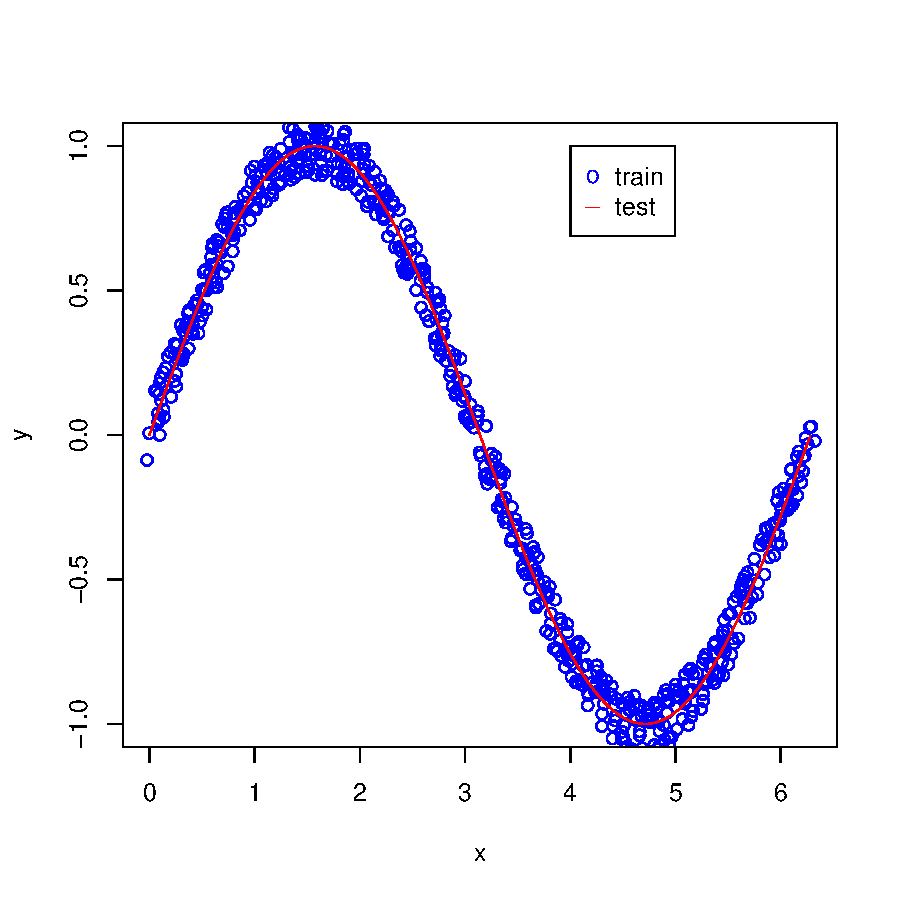
\includegraphics{Relatorio_3-002}

Para realizar o treinamento, os dados foram primeiramente preparados,

\begin{Schunk}
\begin{Sinput}
> x_train <- matrix(x_train, ncol=1)
> y_train <- matrix(y_train, ncol=1)
> x_test <- matrix(x_test, ncol=1)
> y_test <- matrix(y_test, ncol=1)
\end{Sinput}
\end{Schunk}

\noindent
e, como a função de ativação dos neurônios escondidos é tangente hiperbólico, a derivada desta função, $sech^2$, não presente originalmente no R, foi implementada:

\begin{Schunk}
\begin{Sinput}
> sech2 <- function(u){
+     return(((2/(exp(u)+exp(-u)))*(2/(exp(u)+exp(-u)))))
+ }
\end{Sinput}
\end{Schunk}

A função de treinamento do modelo é composta de dois estágios, um de feedfoward, onde o valor de saída é obtido a partir dos valores dos parâmetros de entrada, e outra de backpropagation, onde os pesos são ajustados.

\begin{Schunk}
\begin{Sinput}
> train <- function(x, y, n_neurons=3, tol=0.01, epochs=2000, eta=0.1) {
+ 
+     n_samples <- dim(x)[1]
+ 
+     x_aug <- cbind(replicate(n_samples, 1), x)
+ 
+     features <- dim(x_aug)[2]
+ 
+     # Hidden layer
+     z <- matrix(rnorm(features * n_neurons, 0, 1), ncol=n_neurons)
+ 
+     # Out layer
+     n_out_neurons <- dim(y)[2]
+     new_features <- n_neurons + 1
+     w <- matrix(rnorm(new_features * n_out_neurons, 0, 1), ncol=n_out_neurons)
+ 
+     epoch_errors = c()
+ 
+     model_error <- tol + 1
+     epoch <- 1
+     while (model_error > tol && epoch <= epochs) {
+ 
+         print(paste('Epoch [', epoch, '/', epochs, ']'))
+ 
+         errors = c()
+ 
+         for (index in sample(n_samples)) {
+ 
+             # Feed foward
+             x_in <- x_aug[index,]
+             h <- tanh(x_in %*% z)
+             h_aug <- cbind(1, h)
+             y2 <- h_aug %*% w
+             error <- y[index,] - y2
+ 
+             # Backpropagation
+             w <-w + eta * error[1] * t(h_aug)
+             for (n in seq(dim(z)[2])){
+                 z[,n] <- z[,n] + eta * sech2(sum(x_in * z[, n])) * (error[1] * w[n+1]) * x_in
+             }
+             errors <- c(errors, error)
+         }
+ 
+         model_error <- sum(errors**2) / (n_samples - 1)
+         print(paste("  - Loss (mse):", model_error))
+         epoch_errors <- c(epoch_errors, model_error)
+ 
+         epoch <- epoch + 1
+     }
+ 
+     return (list (
+         'weights' = list(
+             'z' = z,
+             'w' = w
+         ),
+         'epoch_errors' = epoch_errors,
+         'loss' = model_error
+     ))
+ }
\end{Sinput}
\end{Schunk}

Para realizar as predições dos valores de y, conforme o valor de x, foi implementada uma função de predição, da forma:

\begin{Schunk}
\begin{Sinput}
> predict <- function(x, model){
+     z <- model$weights$z
+     w <- model$weights$w
+     n_samples <- dim(x)[1]
+     x_aug <- cbind(replicate(n_samples, 1), x)
+ 
+     y <- matrix(replicate(n_samples, 0), ncol=1)
+ 
+     for (index in seq(n_samples)) {
+ 
+         # Feed foward
+         x_in <- x_aug[index,]
+         h <- tanh(x_in %*% z)
+         h_aug <- cbind(1, h)
+         y[index,] <- (h_aug %*% w)
+     }
+ 
+     return(y)
+ }
\end{Sinput}
\end{Schunk}

\subsection{Execução dos Testes}

O treinamento do modelo, e sua validação foram realizados em 5 testes, onde foram registradas as formas de onda resultantes, e o gráfico dos erros das execuções, da forma:

\begin{Schunk}
\begin{Sinput}
> n_tests <- 5
> mse <- c()
> for (test in seq(n_tests)) {
+     model <- train(x_train, y_train, eta=0.01, n_neurons=3, tol=0.02)
+ 
+     xseq <- seq(length(model$epoch_errors))
+     jpeg(paste0("error_exec_", test, '.jpeg'), width = 350, height = 350)
+ 
+         plot(xseq, model$epoch_errors,
+          type='l',
+          ylim=c(0,max(model$epoch_errors)),
+          main='Train Error',
+          xlab='Epoch',
+          ylab='MSE')
+ 
+     dev.off()
+ 
+     y_predict <- predict(x_test, model)
+ 
+     mse <- c(mse, mean((y_test - y_predict)**2))
+     print(mse)
+ 
+     jpeg(paste0("prediction_exec_", test, '.jpeg'), width = 600, height = 600)
+     plot(x_test,y_test,col='blue',type='l',xlim = c(0,2*pi), ylim = c(-1,1),xlab = 'x',ylab = 'y')
+     par(new=T)
+     plot(x_test,y_predict,col='red',type='l',xlim = c(0,2*pi), ylim = c(-1,1),xlab = 'x',ylab = 'y', main='Prediction Result')
+     legend("topright",
+            c("Original","Predicted"),
+            fill=c("blue","red")
+     )
+     dev.off()
+ }
\end{Sinput}
\end{Schunk}

O erro quadrático médio do modelo, considerando as 5 execuções, é de 0.01806. O gráfico de saída para uma das execuções pode ser visto abaixo:

\begin{figure}[H]
\centering
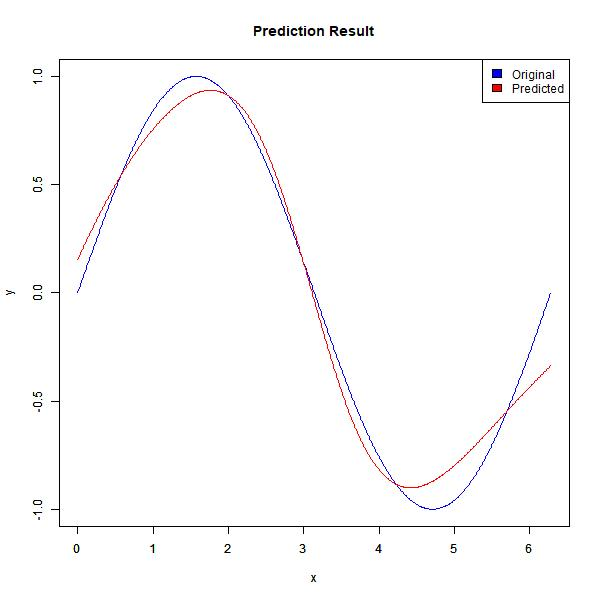
\includegraphics[width=0.7\linewidth]{prediction_exec_4.jpeg}
\end{figure}

\noindent
e a curva de erro de treinamento, por época, para esta execução, foi:

\begin{figure}[H]
\centering
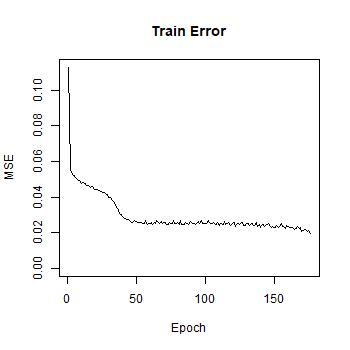
\includegraphics[width=0.7\linewidth]{error_exec_4.jpeg}
\end{figure}

\begin{thebibliography}{1}

	%Each item starts with a \bibitem{reference} command and the details thereafter.
	\bibitem{specificity} % Transaction paper
	ML Metrics: Sensitivity vs. Specificity -
	\url{https://dzone.com/articles/ml-metrics-sensitivity-vs-specificity-difference}.
	Acessado em 28 de agosto de 2019.


\end{thebibliography}

\end{document}
